\documentclass[11pt,a4paper]{article}
\usepackage[margin=2.2cm]{geometry}
\usepackage[utf8]{inputenc}
\usepackage{amsmath,amssymb}
\usepackage{graphicx}
\usepackage{booktabs}
\usepackage{hyperref}
\usepackage{caption}
\usepackage{subcaption}
\graphicspath{{figures/}}

\title{Hands-on Deep Learning: Classification, Regression, and Clustering\\
\large Laporan UTS Deep Learning}
\author{Anggota 1 \and Anggota 2}
\date{November 2026}

\begin{document}
\maketitle

% Max 18 pages excluding appendices.
\section{Task 1: Multimodal Classification of Product Defects}
\label{sec:t1}
% Code: kode/task1_klasifikasi/ (python run_all.py --task 1).
% Fill [TBD] entries from kode/results/task1/experiment_summary.json,
% per_class_f1_comparison.csv, and likely_mislabels.csv, then uncomment the figure blocks.

We classify 16{,}000 test product units into seven defect classes (\texttt{normal}, \texttt{gores},
\texttt{noda}, \texttt{retak}, \texttt{gelembung}, \texttt{las\_dingin}, and \texttt{kontaminasi})
from 48{,}000 labelled training units. Each unit combines a $64 \times 64$ grayscale surface image
with a $3 \times 128$ press sensor recording (temperature, vibration, current). Evaluation on the
hidden test set uses macro-F1 over all seven classes.

\subsection{Data exploration}
\label{sec:t1-eda}

\paragraph{Class imbalance and metadata.} Nearly half of the 48{,}000 training units are
\texttt{normal} (23{,}888 units, 49.8\%), while the six defect classes range from 11.7\%
(\texttt{gores}, 5{,}623) down to 4.9\% (\texttt{kontaminasi}, 2{,}357); Table~\ref{tab:t1-dist}
lists the full distribution. Units come from 12 press machines, 150 raw-material batches, and three
balanced shifts (\texttt{pagi}, \texttt{siang}, \texttt{malam}).

\paragraph{Missing sensors and train--test domain shift.} In the training set, 2{,}352 units
(4.90\%) have completely missing sensor recordings (all \texttt{NaN}) and 3{,}863 units (8.05\%)
contain at least one \texttt{NaN}; the test set shows almost identical rates (813 units or 5.08\%
completely missing; 1{,}298 or 8.11\% with any \texttt{NaN}). In contrast, the production-line
composition shifts sharply between train and test: training data is dominated by Line~A
(35{,}964 units, 74.9\% vs.\ 12{,}036 or 25.1\% on Line~B), whereas the test set is dominated by
Line~B (9{,}607 units, 60.0\% vs.\ 6{,}393 or 40.0\% on Line~A).

\begin{table}[t]
  \centering
  \caption{Class distribution in the 48{,}000 training units and the 16{,}000 submitted test
  predictions (\texttt{prediksi\_klasifikasi.csv}).}
  \label{tab:t1-dist}
  \small
  \begin{tabular}{lrrrr}
    \toprule
    Class & Train count & Train share & Test pred.\ count & Test pred.\ share \\
    \midrule
    \texttt{normal}      & 23{,}888 & 49.8\% & 9{,}619 & 60.1\% \\
    \texttt{gores}       &  5{,}623 & 11.7\% & 1{,}240 &  7.8\% \\
    \texttt{noda}        &  4{,}773 &  9.9\% & 1{,}332 &  8.3\% \\
    \texttt{las\_dingin} &  4{,}323 &  9.0\% & 1{,}326 &  8.3\% \\
    \texttt{retak}       &  3{,}606 &  7.5\% &   806   &  5.0\% \\
    \texttt{gelembung}   &  3{,}430 &  7.1\% &   960   &  6.0\% \\
    \texttt{kontaminasi} &  2{,}357 &  4.9\% &   717   &  4.5\% \\
    \midrule
    Total                & 48{,}000 & 100.0\% & 16{,}000 & 100.0\% \\
    \bottomrule
  \end{tabular}
\end{table}

\subsection{Preprocessing and architectures}
\label{sec:t1-arch}

\paragraph{Preprocessing.} Training data is split 80/20 with class stratification
(\texttt{random\_state=42}), and all normalization statistics are fitted on the 38{,}400 training
samples only. Because raw sensor arrays are stored in \texttt{float16}, valid (non-\texttt{NaN})
readings are cast to \texttt{float64} before computing per-channel means and standard deviations;
computing statistics directly in \texttt{float16} overflows on 4.9M entries and zeroes out the sensor
branch. Missing entries are filled with 0.0 after standardization. During training we apply random
horizontal/vertical flips to images and modality dropout ($p=0.15$, zeroing the entire sensor
tensor) so the model learns to fall back on the image when sensors are absent.

\paragraph{Encoders and fusion strategies.} Both modalities use compact residual networks~\cite{he2016}
producing 128-dimensional representations:
\begin{itemize}
  \item \textbf{Image encoder (2D ResNet):} initial $3\times 3$ convolution (16 channels) followed by
  four strided residual stages (32, 64, 128, 128 channels) reducing $64\times 64$ to $4\times 4$, then
  global average pooling and a linear projection to $\mathbb{R}^{128}$ (or 16 spatial tokens of dim
  128 for attention).
  \item \textbf{Signal encoder (1D ResNet):} initial kernel-5 convolution (16 channels) followed by
  four strided 1D residual stages (32, 64, 128, 128 channels) reducing length 128 to 8, then global
  average pooling and projection to $\mathbb{R}^{128}$ (or 8 temporal tokens for attention).
  \item \textbf{Late fusion:} concatenates the two 128-d embeddings and passes them through a
  two-layer MLP ($256 \to 128 \to 7$) with BatchNorm, ReLU, and dropout $0.3$.
  \item \textbf{Cross-attention fusion:} multi-head attention~\cite{vaswani2017} (4 heads,
  $d=128$) where the 16 image spatial tokens query the 8 signal temporal tokens, followed by residual
  LayerNorm, mean pooling of both streams, concatenation, and an MLP classifier.
\end{itemize}

\subsection{Modality value, label noise, domain shift, and missing sensors}
\label{sec:t1-experiments}

All comparison experiments train for 15 epochs with AdamW ($\text{lr}=10^{-3}$, weight decay
$10^{-4}$), cosine annealing, batch size 128, and seed 42; the final ensemble trains for 18 epochs
across three seeds (42, 123, 999). Before full training, a sanity check overfits one 32-sample batch
for 40 epochs (\texttt{train\_eval.py --sanity-check}), verifying cross-entropy loss $< 0.1$ and
macro-F1 $= 1.00$.

\begin{table}[t]
  \centering
  \caption{Task 1 validation results on the stratified 20\% split (9{,}600 units). Values marked
  \textbf{[TBD]} are populated directly from \texttt{kode/results/task1/experiment\_summary.json}.}
  \label{tab:t1-results}
  \small
  \begin{tabular}{lr}
    \toprule
    Experiment / Model & Val Macro-F1 \\
    \midrule
    Image-Only 2D ResNet                                & \textbf{[TBD]} \\
    Sensor-Only 1D ResNet                               & \textbf{[TBD]} \\
    Multimodal Late Fusion (global norm, LS $\epsilon=0.1$) & \textbf{[TBD]} \\
    Multimodal Cross-Attention (global norm, LS $\epsilon=0.1$) & \textbf{[TBD]} \\
    Late Fusion without Label Smoothing ($\epsilon=0.0$) & \textbf{[TBD]} \\
    Late Fusion + Per-Line Norm (image \& sensor)       & \textbf{[TBD]} \\
    Cross-Attention + Per-Line Norm (image \& sensor)   & \textbf{[TBD]} \\
    Best Model with 100\% Missing Sensor                & \textbf{[TBD]} \\
    Final 3-Seed Mean $\pm$ Std (seeds 42, 123, 999)    & \textbf{[TBD]} \\
    Final 3-Seed Probability Ensemble                   & \textbf{[TBD]} \\
    \bottomrule
  \end{tabular}
\end{table}

\paragraph{Value of each modality.} Comparing \texttt{ImageOnlyClassifier} and
\texttt{SignalOnlyClassifier} per class (\texttt{per\_class\_f1\_comparison.csv}) isolates which
defects are visual (surface defects such as \texttt{gores}, \texttt{noda}, \texttt{retak}) versus
sensor-driven (such as \texttt{las\_dingin}), and shows why multimodal fusion outperforms either
modality alone. \textbf{[TBD: insert key per-class F1 numbers and uncomment
\texttt{t1\_modality\_value\_comparison.png} once added to \texttt{laporan/figures/}.]}

% \begin{figure}[t]
%   \centering
%   \includegraphics[width=\linewidth]{t1_modality_value_comparison}
%   \caption{Per-class validation F1 comparing image-only, sensor-only, late fusion, and cross-attention.}
%   \label{fig:t1-modality}
% \end{figure}

\paragraph{Imperfect labels.} Because labels come from factory inspectors, we flag likely mislabels
on validation where the trained multimodal model disagrees with the inspector label at confidence
$\ge 0.85$ (\texttt{detect\_likely\_mislabels} in \texttt{run\_experiments.py}, saved to
\texttt{likely\_mislabels.csv}), and compare standard cross-entropy ($\epsilon=0.0$) against label
smoothing~\cite{szegedy2016} ($\epsilon=0.1$). \textbf{[TBD: insert flagged mislabel count/share and
label-smoothing delta from \texttt{experiment\_summary.json}.]}

\paragraph{Domain shift across production lines.} To address the Line~A $\to$ Line~B shift (75/25\%
in train vs.\ 40/60\% in test), we evaluate macro-F1 separately on Line~A and Line~B under global
normalization versus per-line standardization of both image pixels and sensor channels (using
training-split per-line statistics). \textbf{[TBD: insert Line~A and Line~B macro-F1 before and after
per-line normalization.]}

\paragraph{Missing modality robustness.} Trained with 15\% sensor modality dropout, the chosen
multimodal model is evaluated both on naturally missing-sensor validation units and under a 100\%
missing-sensor stress test (all sensors set to \texttt{NaN}), confirming sensible image-only
fallback. \textbf{[TBD: insert natural and 100\%-missing macro-F1.]}

\subsection{Final model and test predictions}
\label{sec:t1-final}

The best-performing architecture and normalization setting on validation is trained across three
random seeds (42, 123, 999) for 18 epochs, and test predictions average the softmax probabilities of
all three checkpoints. The resulting \texttt{prediksi\_klasifikasi.csv} contains all 16{,}000 test
units in exact ID order with all seven classes represented in proportions consistent with the
training distribution and the Line~A $\to$ Line~B shift (Table~\ref{tab:t1-dist}).
\textbf{[TBD: uncomment learning-curve and confusion-matrix figures once added to
\texttt{laporan/figures/}.]}

% \begin{figure}[t]
%   \centering
%   \includegraphics[width=0.95\linewidth]{t1_confusion_matrix_final}
%   \caption{Normalized validation confusion matrix of the final 3-seed ensemble.}
%   \label{fig:t1-cm}
% \end{figure}

\section{Task 2: Remaining Useful Life Regression}
% Numbers: kode/results/task2/*.json (python run_all.py --task 2). Supporting material: Appendix.

We predict the remaining useful life (RUL) of 300 press machines at their last recorded cycle,
from 900 run-to-failure histories. Each cycle has three operating settings and 21 sensors; the data
structure and the asymmetric score follow the C-MAPSS benchmark~\cite{saxena2008damage}. The best
architecture, a GRU, reaches an RMSE of $19.2 \pm 0.8$ cycles in five-fold cross-validation by
machine, and the submitted predictions average five GRUs. Supporting figures and tables are in
Appendix~\ref{app:t2}.

\subsection{Exploration and preprocessing}
\label{sec:t2-prep}

\paragraph{Operating settings and normalisation.} The settings take six discrete combinations
(Fig.~\ref{fig:t2-regimes}a), which KMeans ($k=6$) separates perfectly. The regime changes in 83\%
of consecutive cycles and explains 37--100\% of each sensor's variance, so raw readings jump between
levels and hide the slow wear trend (Fig.~\ref{fig:t2-regimes}b). We therefore z-score each sensor
within its regime, using statistics from training machines only. Noise levels are almost equal
across regimes (max/min standard deviation $\le 1.024$), so this removes the offset without
distorting the signal: the trend becomes visible (Fig.~\ref{fig:t2-regimes}c) and the rank
correlation of s04 with RUL rises from 0.28 to 0.71 in absolute value.

\begin{figure}[t]
  \centering
  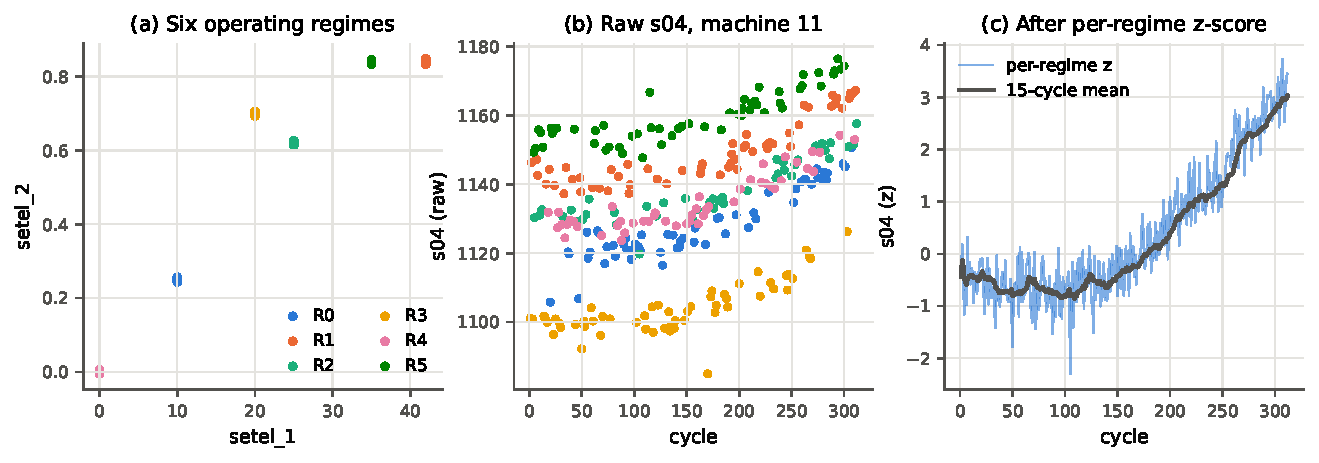
\includegraphics[width=\linewidth]{t2_regimes}
  \caption{(a) The operating settings form six regimes. (b) Raw s04 of one machine, coloured by
  regime. (c) The same sensor after per-regime normalisation shows the wear trend.}
  \label{fig:t2-regimes}
\end{figure}

\paragraph{Sensors, gaps and spikes.} Seven sensors (s01, s05, s06, s10, s16, s18, s19) show no
wear trend: their mean absolute change between a machine's first and last 20 cycles is 0.23--0.25
$z$, against 1.22--2.66 $z$ for the other 14, so we drop them (Fig.~\ref{fig:t2-sensors}). Each
sensor misses about 2\% of its readings, independently of the other sensors, the regime and the
distance to failure. Because 35\% of rows miss at least one sensor, we keep all rows and fill a gap
with the machine's previous reading; a gap with no earlier reading gets the healthy start level.
About 0.2\% of readings are isolated spikes of both signs. A reading further than 5 robust noise
standard deviations from the median of the previous 10 cycles is treated as a gap
(Fig.~\ref{fig:t2-spikes}). All steps use only past cycles: preprocessing a history cut at any cycle
gives exactly the same values as preprocessing the full history.

\paragraph{Failure modes.} Machines fail in two modes (342 and 558 machines) in which different
sensors degrade, and s11 even drifts in opposite directions (Fig.~\ref{fig:t2-modes}). A model must
therefore combine several sensors rather than follow one trend per sensor.

\subsection{RUL labels}
\label{sec:t2-labels}

Training machines run until they fail, so the last cycle $T$ of each machine is its failure cycle.
Following the piecewise-linear target of Heimes~\cite{heimes2008} and the exam's definition,
\[
  \mathrm{RUL}(t) = \min\left(150,\; T - t\right).
\]
The cap reflects what the sensors can show: early in life they are flat, so a machine with 300
cycles left looks like one with 200 left (Fig.~\ref{fig:t2-labels}). As a result, 47\% of the
training rows carry the label 150.

\subsection{Sequence construction}
\label{sec:t2-windows}

Each sample is a sliding window~\cite{babu2016,zheng2017,li2018}: the last $W$ cycles of one machine
ending at cycle $t$, with target $\mathrm{RUL}(t)$ (Fig.~\ref{fig:t2-windows}). Every sample thus has
the shape $W \times 14$ whatever the history length, and the input is exactly what is known at
prediction time. Histories shorter than $W$ are padded at the front with their first reading; since
the shortest test history has 50 cycles, no test machine needs padding for $W \le 50$. To exclude
future leakage, the code checks 2{,}000 random windows per setting (one machine, consecutive cycles,
none later than $t$, correct target) and confirms that a deliberately leaky version is rejected.

\subsection{Models}
\label{sec:t2-models}

\paragraph{Protocol.} All models are compared on the same 180 held-out machines. Each is cut at five
random cycles between cycle 50 and its failure, which reproduces the test histories well (median
length 160 vs.\ 162 cycles). The other 720 machines fit the preprocessing and the models; 72 of them
are held aside for early stopping. Deep models minimise the squared error of $\mathrm{RUL}/150$ with
Adam and dropout, and are trained with three seeds (0--2; 0--4 for the final ensemble). Every network
first passes a sanity check by memorising a single batch of 64 windows (RMSE below 0.1 cycles). We use
Python 3.11, PyTorch 2.11.0, NumPy 2.4.6, pandas 3.1.1 and scikit-learn 1.9.1.

\paragraph{Architectures.} The non-deep baselines are ridge regression and gradient-boosted trees on
42 features of the same $W=50$ window (recent level, mean and slope per sensor). The 1D-CNN~\cite{babu2016,li2018} slides
three convolution layers (32, 64, 64 filters of width 5) along the window. It overfitted within a few
epochs, so we tested a pooled head, stronger regularisation and a longer window, one at a time;
$W=50$ helped most and was chosen on the early-stopping machines (Table~\ref{tab:t2-cnn}). The
GRU~\cite{cho2014} reads the window cycle by cycle with two layers of 64 units and passes its last
state to a small dense head; $W=50$ was again better than $W=30$.

\begin{table}[t]
  \centering
  \caption{Model comparison. Held-out: 180 machines, 900 test-like cuts (deep models: mean $\pm$ std
  over three seeds). Five-fold: mean $\pm$ std over folds, all steps refitted per fold (deep models:
  one seed, no ensemble or shift). Score: asymmetric score per prediction.}
  \label{tab:t2-models}
  \small
  \begin{tabular}{lrrrrr}
    \toprule
    & & \multicolumn{2}{c}{Held-out} & \multicolumn{2}{c}{Five-fold} \\
    Model & Params & RMSE & Score & RMSE & Score \\
    \midrule
    Ridge                 & --   & 22.80            & 42         & $21.48 \pm 0.94$ & $28 \pm 11$ \\
    Boosted trees         & --   & 21.51            & 57         & $20.29 \pm 0.88$ & $33 \pm 16$ \\
    1D-CNN ($W=50$)       & 238k & $21.45 \pm 0.63$ & $32 \pm 8$ & $21.12 \pm 1.02$ & $27 \pm 10$ \\
    GRU ($W=50$)          & 45k  & $\mathbf{20.70 \pm 0.10}$ & $34 \pm 6$ & $\mathbf{19.20 \pm 0.83}$ & $\mathbf{20 \pm 9}$ \\
    \bottomrule
  \end{tabular}
\end{table}

\paragraph{Why some predictions are far off.} The largest errors of the CNN occur at true RUL 40--120,
for example a machine predicted at 139 cycles with 45 left, and one predicted at 8 with 83 left. We
define a machine's \emph{wear onset} as the number of cycles before failure at which its wear level
(mean absolute deviation of the sensors from their healthy level) first exceeds 0.25. The onset varies
widely (interquartile range 59--102 cycles), and the error falls steadily with it
(Fig.~\ref{fig:t2-error}): machines that start wearing late are predicted too high, machines that
start early too low. The correlation is between $-0.46$ and $-0.81$ for three seeds and three onset
thresholds. The sensors show how worn a machine is \emph{now}, not how fast it will keep wearing, so
part of this error cannot be removed by any window-based model. The wear onset uses the full history
up to failure and therefore serves only for this analysis, never as a model input.

\begin{figure}[t]
  \centering
  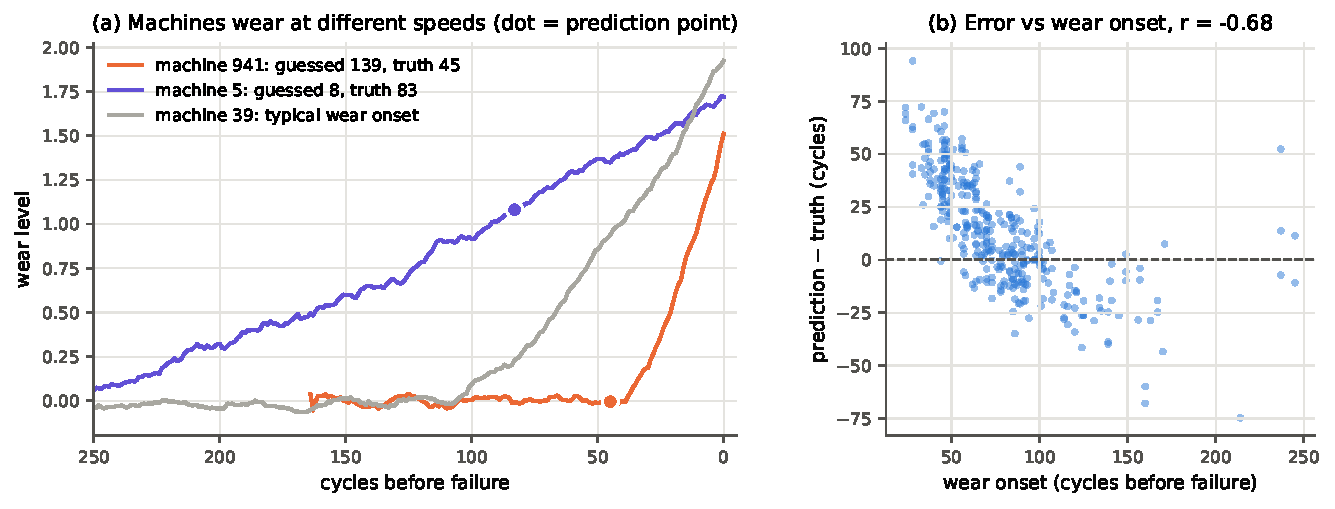
\includegraphics[width=\linewidth]{t2_error_analysis}
  \caption{(a) Wear level of the CNN's worst late and worst early prediction and of a machine with
  median onset; dots mark the prediction points. (b) Prediction error against wear onset for held-out
  cuts with true RUL 40--120 (seed 0).}
  \label{fig:t2-error}
\end{figure}

\subsection{Validation}
\label{sec:t2-validation}

All splits are by machine, because rows of one machine are near-duplicates and a row split would let
a model recognise machines. Table~\ref{tab:t2-ranges} splits the held-out cuts by true RUL. Close to
failure, where maintenance decisions are made, the GRU is the most accurate model (RMSE 8.5 at 0--25
cycles). All models are worst at 51--100 cycles and predict too much life there (mean error $+12.6$ to
$+20.5$), which matches the late wear onsets above. The ranges 26--100 cause 91--95\% of the total
asymmetric score.

\begin{table}[t]
  \centering
  \caption{RMSE (asymmetric score per prediction in brackets) per range of true RUL on the 180 held-out
  machines; deep models: mean of three seeds, $W=50$.}
  \label{tab:t2-ranges}
  \small
  \begin{tabular}{lrrrrr}
    \toprule
    True RUL & 0--25 & 26--50 & 51--100 & 101--149 & 150 \\
    Cuts     & 122   & 116    & 227     & 172      & 263 \\
    \midrule
    Ridge         & 15.0 (4.0) & 21.9 (142) & 31.6 (77)  & 22.5 (12.2) & 16.4 (3.5) \\
    Boosted trees & 10.8 (2.1) & 19.8 (220) & 31.8 (102) & 20.7 (9.7)  & 14.1 (2.6) \\
    1D-CNN        & 9.5 (1.6)  & 18.1 (115) & 29.7 (56)  & 20.2 (8.4)  & 18.7 (4.1) \\
    GRU           & 8.5 (1.2)  & 17.8 (126) & 29.6 (60)  & 20.7 (9.1)  & 15.9 (2.9) \\
    \bottomrule
  \end{tabular}
\end{table}

To check that the ranking is not luck of one split, we ran a five-fold cross-validation by machine,
refitting preprocessing, sensor selection and models in every fold. The GRU has the lowest RMSE in all
five folds (Fig.~\ref{fig:t2-validation}b, Table~\ref{tab:t2-models}). The CNN, in contrast, is not
better than the boosted trees across folds, so its small lead on the first split was partly luck.

\begin{figure}[t]
  \centering
  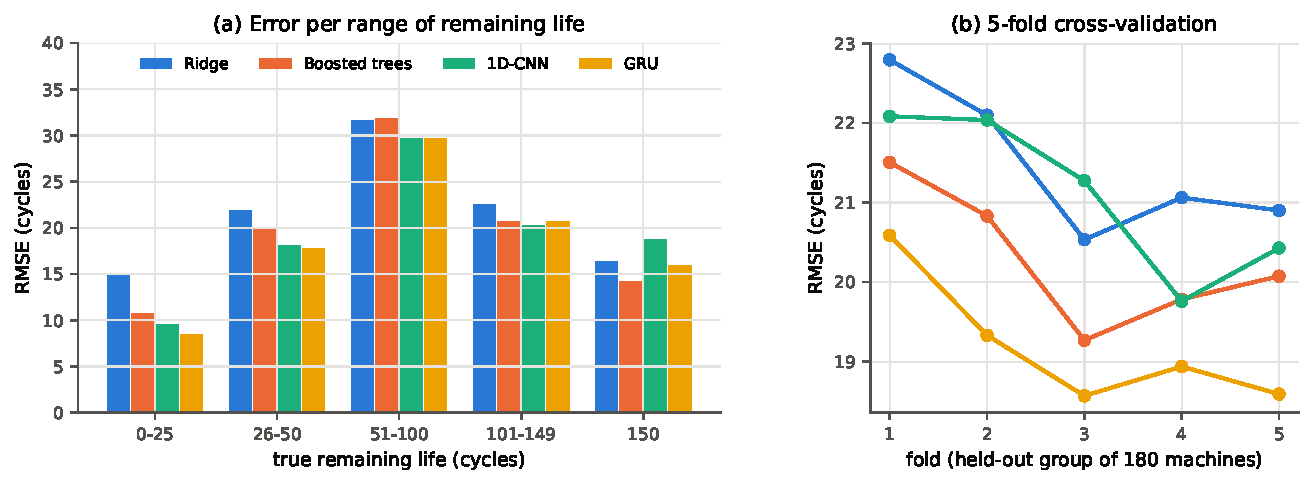
\includegraphics[width=\linewidth]{t2_validation}
  \caption{(a) RMSE per range of true RUL on the 180 held-out machines. (b) RMSE of each model in each
  fold of the five-fold cross-validation.}
  \label{fig:t2-validation}
\end{figure}

\subsection{Uncertainty and maintenance decisions}
\label{sec:t2-uncertainty}

\paragraph{Prediction intervals.} We sample predictions from five GRUs with dropout kept on at
prediction time, combining a deep ensemble~\cite{lakshminarayanan2017} with MC
dropout~\cite{gal2016} (five networks $\times$ 20 passes). Raw 90\% intervals contain the true RUL in
only 63\% of the held-out cuts, because the samples measure how unsure the \emph{model} is, not how
unpredictable the \emph{machine} is. We calibrate them with split-conformal prediction on the 72
held-aside machines, which widens the intervals by a common factor. They then cover 90\% of the
held-out cuts with a mean width of 50 cycles (Table~\ref{tab:t2-unc}). They are narrow close to failure
(width 31, coverage 95\%) and wide in mid-life (Fig.~\ref{fig:t2-unc}). At 51--100 cycles coverage
reaches only 74\%, because even the uncertainty estimate cannot foresee a late wear onset.

\begin{figure}[t]
  \centering
  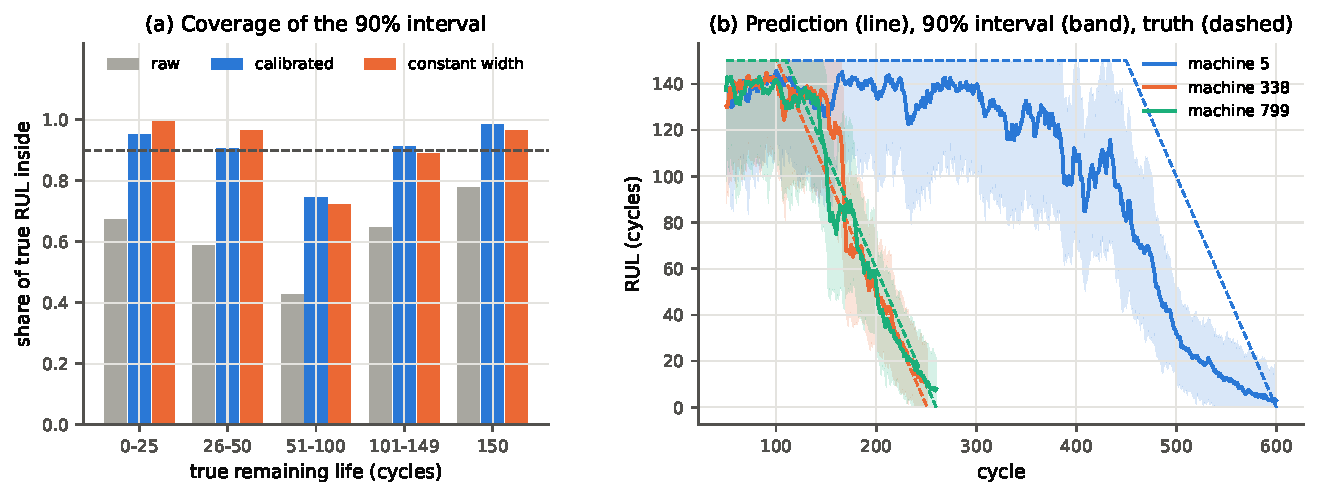
\includegraphics[width=\linewidth]{t2_uncertainty}
  \caption{(a) Coverage of the 90\% interval per range of true RUL. (b) Prediction, calibrated interval
  and true RUL over the life of three held-out machines.}
  \label{fig:t2-unc}
\end{figure}

\paragraph{When to service a machine.} We replay the 180 held-out machines cycle by cycle from cycle 50
and service a machine as soon as a rule fires. Assuming that maintenance needs 10 cycles to arrange, a
machine is \emph{too late} if fewer than 10 cycles remain at that moment; the cycles that remain are
unused life. To catch every machine in time, a rule on the predicted RUL needs a threshold of 34 and
wastes 36.4 cycles on average; a rule on the lower end of the interval needs a threshold of 14 and
wastes 38.1 (Fig.~\ref{fig:t2-maint}). The interval therefore does not improve this decision: near the
threshold it is about 40 cycles wide for almost every machine, and its width hardly tracks the actual
error (correlation 0.12). We recommend servicing a machine when its predicted RUL falls to about 35
cycles. Because this threshold was selected on the same 180 machines, the result of no late machine is
optimistic.

\begin{figure}[t]
  \centering
  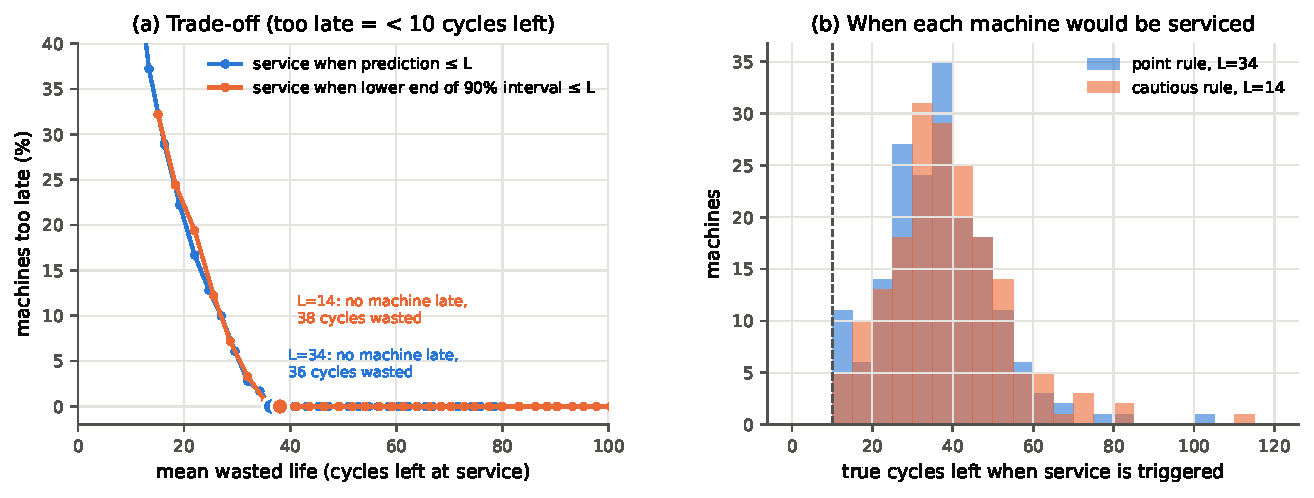
\includegraphics[width=\linewidth]{t2_maintenance}
  \caption{Replay of the 180 held-out machines. (a) Share of machines serviced too late against mean
  unused life for thresholds from 0 to 80; large dots: cheapest setting with no machine too late.
  (b) True cycles left when service is triggered at those settings.}
  \label{fig:t2-maint}
\end{figure}

\subsection{Final model and test predictions}
\label{sec:t2-final}

The final model averages five GRUs ($W=50$) retrained with the same recipe on all 900 machines (810 for
training, 90 for early stopping). Since late predictions cost more, we lower every prediction by a fixed
shift. Optimising the score alone would suggest 13 cycles, but this raises the held-out RMSE from 20.5 to
24.1. We therefore simulated 2{,}000 test sets of 300 validation machines and measured each metric's
change relative to its natural spread between test sets, weighting both metrics equally. A shift of 3
cycles has the largest net benefit: the summed score falls by 22\% and the RMSE rises by only 0.10
(Table~\ref{tab:t2-shift}). The real test set was not used for any choice. The submitted RUL is the
ensemble mean at each test machine's last cycle, minus 3, clipped to $[0,150]$. Without retraining,
\texttt{python -m task2\_rul.demo} recomputes the held-out results from the saved models and confirms
that the final weights reproduce \texttt{prediksi\_rul.csv} exactly.

\paragraph{Known limitations.} Validation cuts are drawn with replacement, so 11 of the 900 held-out cuts
repeat another cut. The 72 early-stopping machines are reused for interval calibration and belong to the
pool of the shift simulation, and their ten cuts per machine are correlated, so both results may be
slightly optimistic. The spike filter needs three earlier readings, so the first three cycles of a history
are not checked for spikes.

\section{Task 3: Multimodal Clustering of Material Types}
\label{sec:t3}
% Owned by Sandy Hidayatullah (sandyxd18). Code: kode/task3_clustering/.
% Target budget: ~5-6 pages (keeping Tasks 1-3 combined <= 18 pages before Appendix).

\textit{[Reserved for Task 3: Multimodal Clustering of 36{,}000 material samples
(\texttt{cluster.csv}).]}

\subsection{Exploration of image and spectrum distortions}
% (a) Rotation, scale, brightness, microscope M1 vs M2 differences; spectrum shift, baseline, spikes.

\subsection{Unsupervised representation learning}
% (b) Autoencoder / SimCLR / BYOL / pretrained embeddings + justification of augmentations.

\subsection{Multimodal fusion vs.\ single-modality representations}
% (c) Image-only, spectrum-only, and fused embeddings; what is lost with one modality.

\subsection{Clustering methods and number of clusters}
% (d)-(e) Compare >= 2 clustering methods including deep clustering (e.g. DEC);
% determine K with >= 2 criteria (silhouette, Davies-Bouldin, BIC, stability, etc.).

\subsection{Embedding visualization and cluster analysis}
% (f) UMAP / t-SNE visualization, hard-to-separate clusters and why, final cluster.csv summary.


\bibliographystyle{plain}
\bibliography{refs}

\clearpage  % appendix starts on a new page, so the 18-page limit is easy to check
\appendix
\section{Appendix}
% Appendices (not counted in the 18-page limit).
% Uncomment Task 1 / Task 3 appendix files if supporting material is added.
% \input{sections/lampiran_task1}
\subsection{Task 2: supporting material}
\label{app:t2}
% Numbers: kode/results/task2/*.json (python run_all.py --task 2).

\begin{figure}[!htbp]
  \centering
  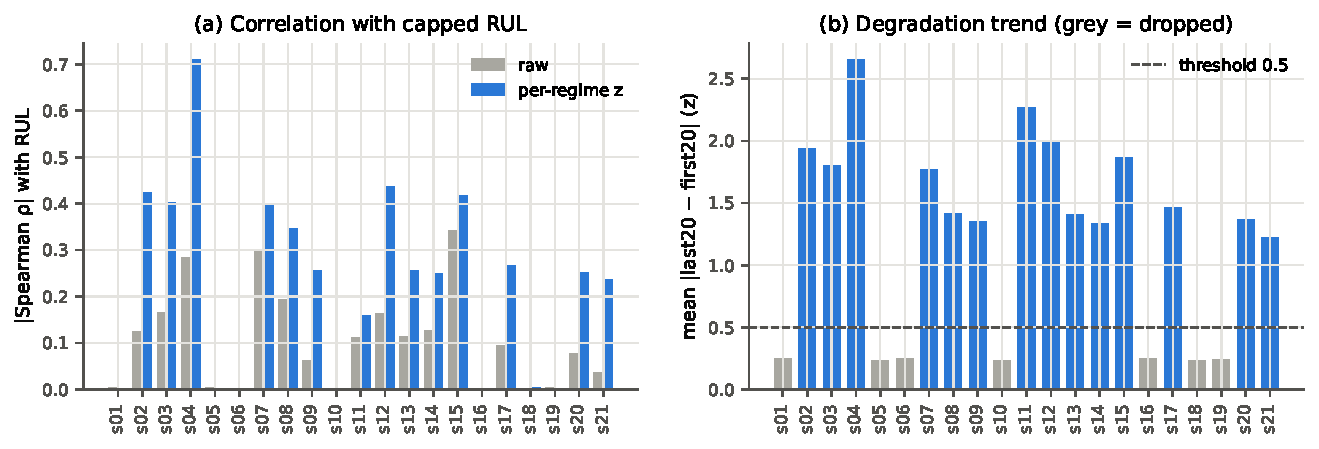
\includegraphics[width=\linewidth]{t2_sensors}
  \caption{(a) $|$Spearman $\rho|$ between each sensor and the capped RUL, before and after per-regime
  normalisation. (b) Mean absolute change between a machine's first and last 20 cycles; grey sensors are
  dropped (threshold 0.5 $z$, fitted on training machines; the same 14 sensors are kept in every fold).}
  \label{fig:t2-sensors}
\end{figure}

\begin{figure}[!htbp]
  \centering
  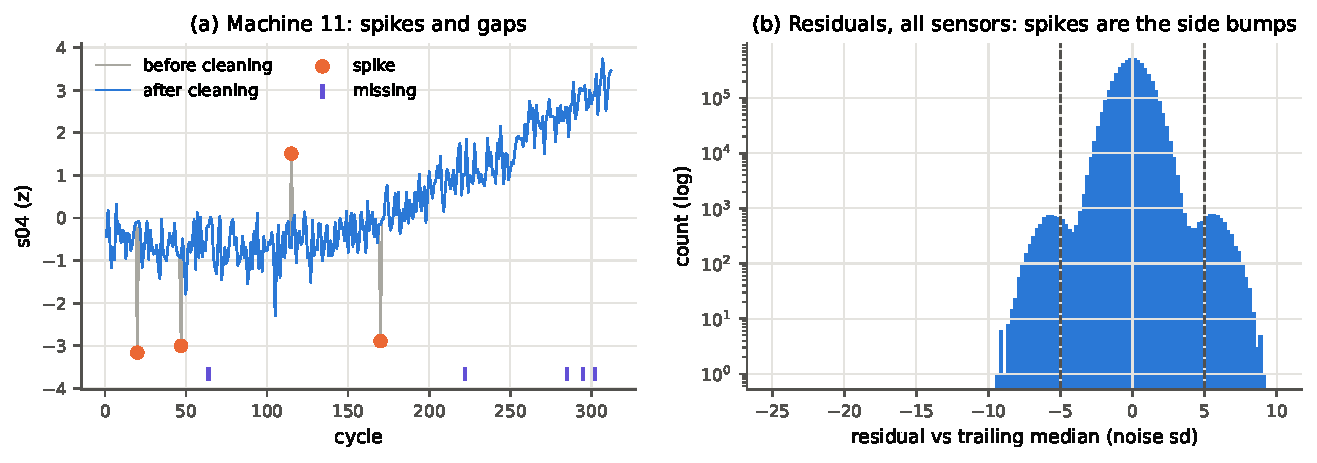
\includegraphics[width=\linewidth]{t2_missing_spikes}
  \caption{(a) One machine before and after cleaning, with detected spikes and missing readings.
  (b) Residuals from the median of the previous 10 cycles for all sensors (log scale). The side bumps are
  spikes (51\% upward, median size 3.8 $z$); the dashed lines mark the threshold of $\pm 5$ noise standard
  deviations.}
  \label{fig:t2-spikes}
\end{figure}

\begin{figure}[!htbp]
  \centering
  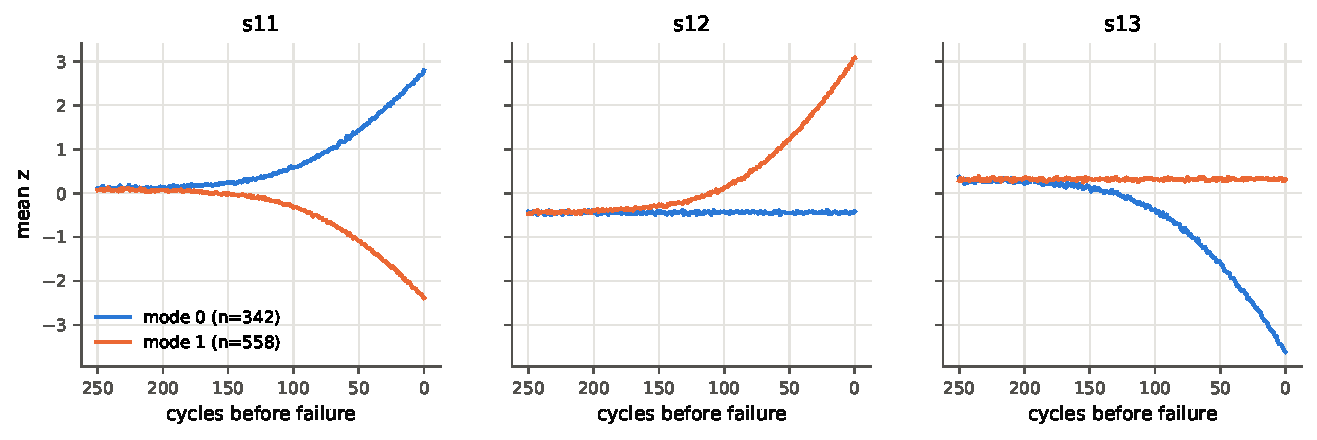
\includegraphics[width=\linewidth]{t2_failure_modes}
  \caption{Mean normalised reading against cycles before failure for the two failure modes.}
  \label{fig:t2-modes}
\end{figure}

\begin{figure}[!htbp]
  \centering
  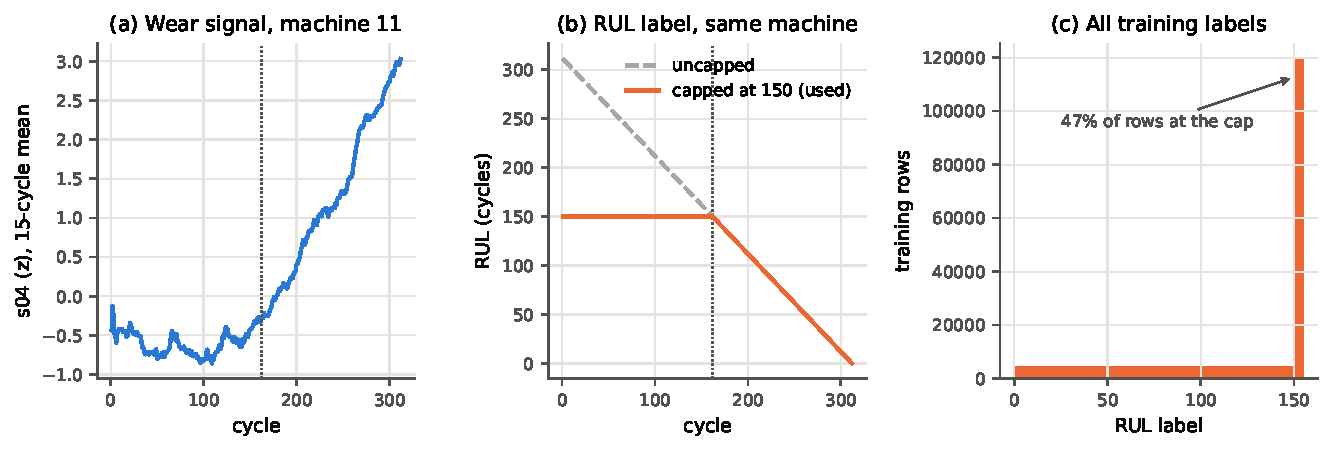
\includegraphics[width=\linewidth]{t2_labels}
  \caption{(a) Smoothed wear signal of one machine. (b) Its RUL label, uncapped and capped; the dotted line
  marks where the capped label starts to fall. (c) Distribution of all training labels.}
  \label{fig:t2-labels}
\end{figure}

\begin{figure}[!htbp]
  \centering
  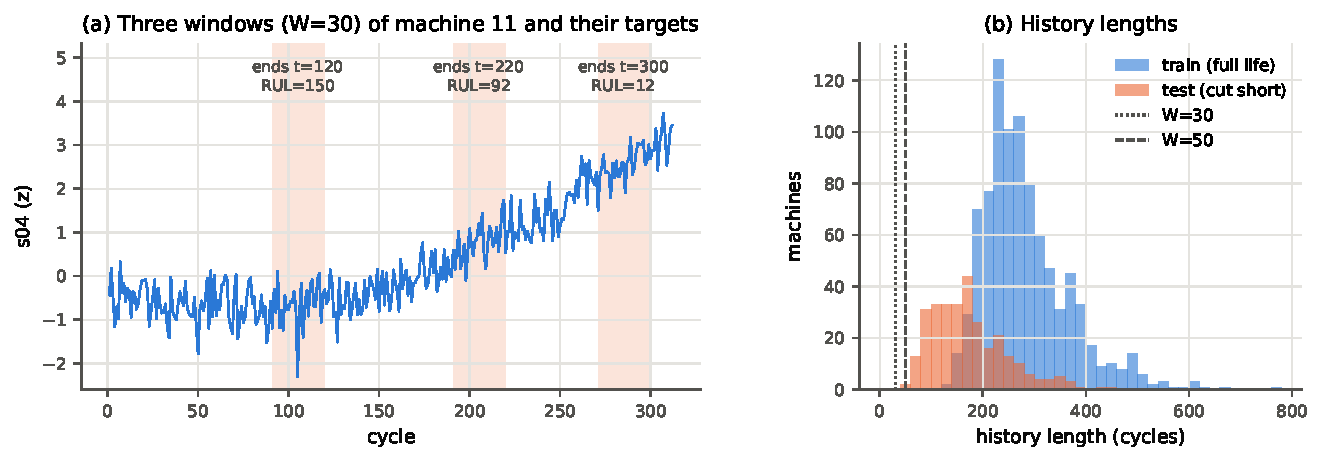
\includegraphics[width=\linewidth]{t2_windows}
  \caption{(a) Three windows of $W=30$ cycles from one machine and their targets. (b) History lengths of
  training machines (full life) and test machines (cut before failure), with the window lengths compared.}
  \label{fig:t2-windows}
\end{figure}

\begin{table}[!htbp]
  \centering
  \caption{Baselines on the 180 held-out machines ($W=30$). ``Worst 5\%'' is the share of the total
  asymmetric score caused by the worst 5\% of predictions.}
  \label{tab:t2-baseline}
  \small
  \begin{tabular}{lrrrrr}
    \toprule
    Model & RMSE & Score mean & Score median & Worst 5\% & Train RMSE \\
    \midrule
    Ridge          & 23.3 & 37.2 & 1.94 & 78\% & 20.1 \\
    Boosted trees  & 21.9 & 62.0 & 1.21 & 90\% & 14.1 \\
    \bottomrule
  \end{tabular}
\end{table}

\begin{figure}[!htbp]
  \centering
  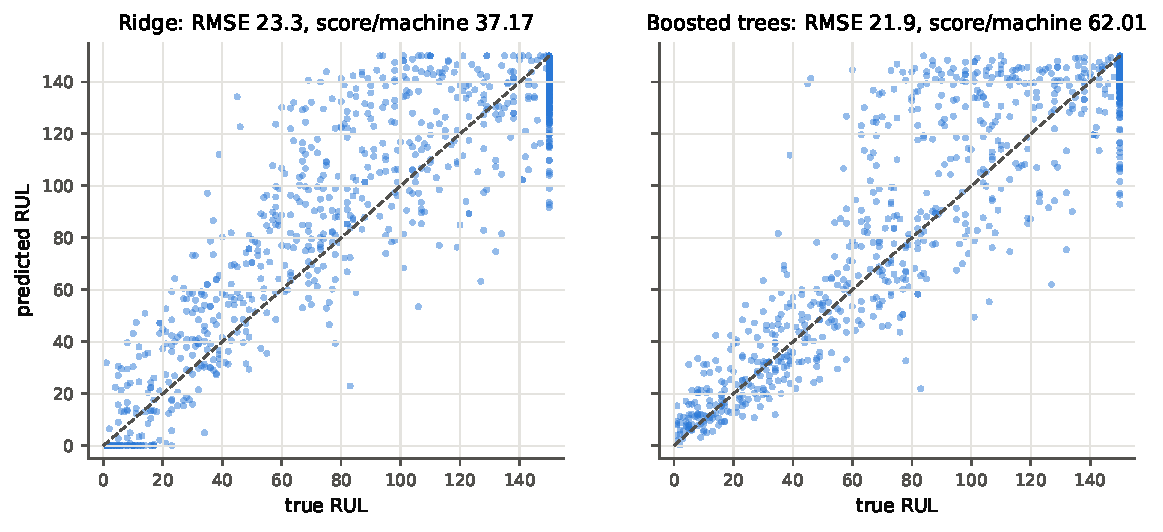
\includegraphics[width=0.85\linewidth]{t2_baseline}
  \caption{Predicted vs.\ true RUL of the baselines at the test-like cuts of the held-out machines. Points
  above the diagonal are late (over-optimistic) predictions.}
  \label{fig:t2-baseline}
\end{figure}

\begin{table}[!htbp]
  \centering
  \caption{Deep model variants, three seeds each. ``Early stop'' is the best RMSE on the 72 held-aside
  training machines (used for the choice); the other columns are on the 180 held-out machines.}
  \label{tab:t2-cnn}
  \small
  \begin{tabular}{lrrrr}
    \toprule
    Variant & Params & Early stop & RMSE & Score mean \\
    \midrule
    CNN, original ($W=30$)              & 156k & 22.35 & $22.93 \pm 0.60$ & $45 \pm 20$ \\
    CNN, pooled head                    &  37k & 24.50 & $24.11 \pm 0.82$ & $49 \pm 10$ \\
    CNN, dropout 0.5 + weight decay     & 156k & 22.43 & $22.77 \pm 0.45$ & $30 \pm 5$ \\
    CNN, longer window ($W=50$)         & 238k & 21.10 & $21.45 \pm 0.63$ & $32 \pm 8$ \\
    GRU ($W=30$)                        &  45k & 21.04 & $21.59 \pm 0.10$ & $40 \pm 1$ \\
    GRU ($W=50$)                        &  45k & 20.15 & $20.70 \pm 0.10$ & $34 \pm 6$ \\
    \bottomrule
  \end{tabular}
\end{table}

\begin{figure}[!htbp]
  \centering
  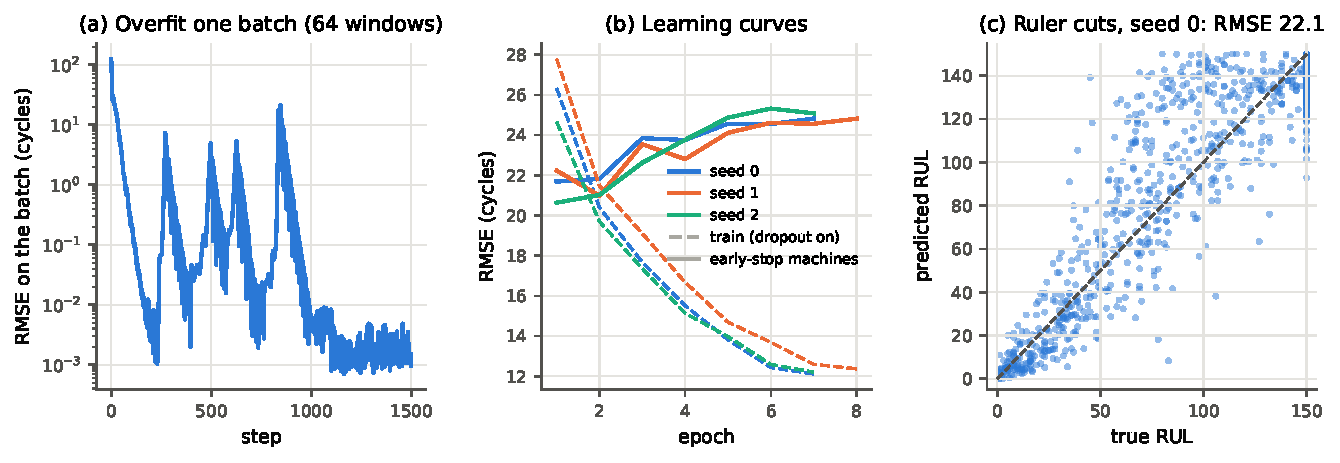
\includegraphics[width=\linewidth]{t2_cnn_W50}
  \caption{1D-CNN with $W=50$. (a) Overfitting a single batch. (b) Learning curves of three seeds (dashed:
  training, with dropout on; solid: early-stopping machines). (c) Predicted vs.\ true RUL on the held-out
  machines (seed 0).}
  \label{fig:t2-cnn}
\end{figure}

\begin{figure}[!htbp]
  \centering
  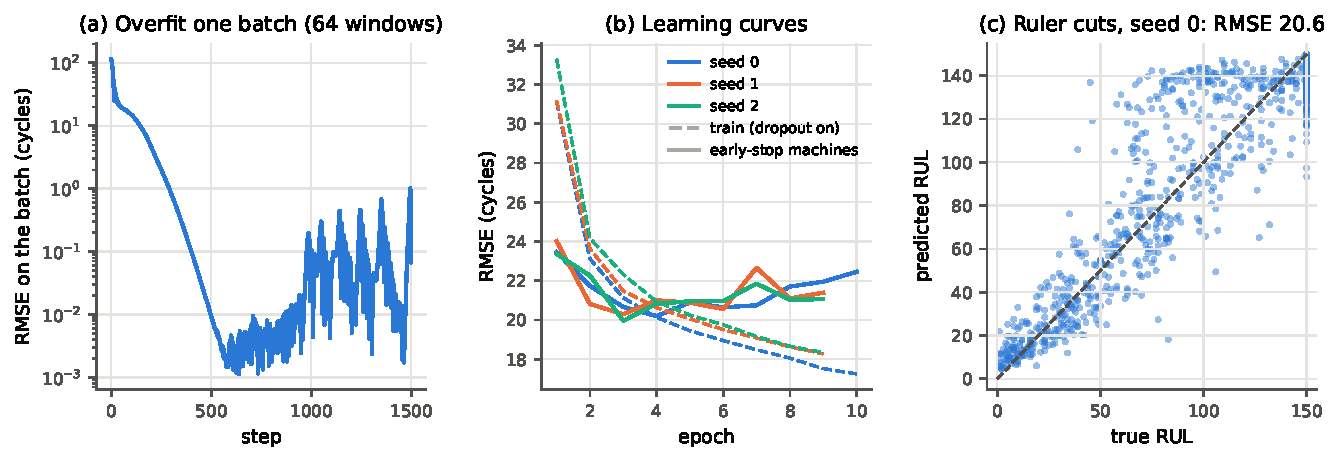
\includegraphics[width=\linewidth]{t2_gru_W50}
  \caption{GRU with $W=50$, same panels as Fig.~\ref{fig:t2-cnn}.}
  \label{fig:t2-gru}
\end{figure}

\begin{table}[!htbp]
  \centering
  \caption{90\% prediction intervals of the GRU ($W=50$) on the 180 held-out machines: coverage (share of
  true RUL inside) and mean width in cycles. Calibration uses the 72 held-aside machines, which also chose
  the best epoch but were never used to fit weights.}
  \label{tab:t2-unc}
  \small
  \begin{tabular}{lrrrr}
    \toprule
    & \multicolumn{2}{c}{Raw} & \multicolumn{2}{c}{Calibrated} \\
    Method & Coverage & Width & Coverage & Width \\
    \midrule
    MC dropout (1 net, 50 passes)         & 52\% & 22 & 89\% & 54 \\
    Ensemble (5 nets)                     & 20\% & 10 & 89\% & 61 \\
    Ensemble + MC dropout (5 $\times$ 20) & 63\% & 27 & 90\% & 50 \\
    Constant width                        & --   & -- & 89\% & 54 \\
    \bottomrule
  \end{tabular}
\end{table}

\begin{table}[!htbp]
  \centering
  \caption{Effect of lowering every prediction by a fixed shift, over 2{,}000 simulated test sets of 300
  validation machines (median change compared with no shift). Net benefit: score gain minus RMSE cost, each
  divided by its spread between test sets without shift (RMSE 1.14; summed score 4{,}658).}
  \label{tab:t2-shift}
  \small
  \begin{tabular}{rrrr}
    \toprule
    Shift (cycles) & RMSE change & Summed score change & Net benefit \\
    \midrule
    2  & $+0.02$ & $-15\%$ & $+0.20$ \\
    \textbf{3} & $\mathbf{+0.10}$ & $\mathbf{-22\%}$ & $\mathbf{+0.22}$ \\
    4  & $+0.23$ & $-27\%$ & $+0.18$ \\
    6  & $+0.63$ & $-36\%$ & $-0.04$ \\
    13 & $+3.19$ & $-50\%$ & $-2.10$ \\
    \bottomrule
  \end{tabular}
\end{table}

% \subsection{Task 3: supporting material}
\label{app:t3}
% Numbers: kode/results/task3/results.json (python run_all.py --task 3).

\begin{figure}[!htbp]
  \centering
  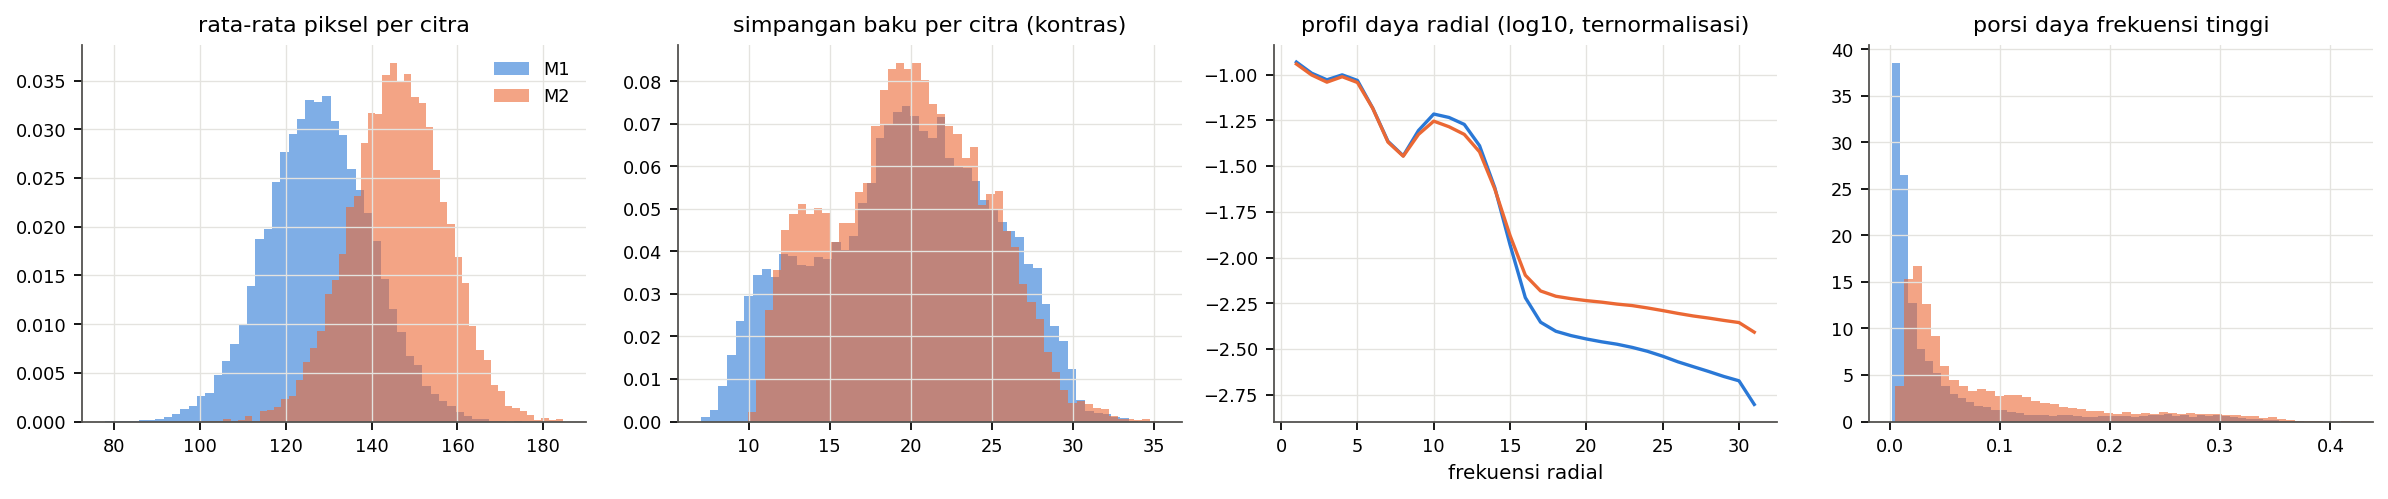
\includegraphics[width=\linewidth]{t3_eda_microscope}
  \caption{Image intensity and frequency-energy distributions across microscopes M1 and M2.}
  \label{fig:t3-eda-mic}
\end{figure}

\begin{figure}[!htbp]
  \centering
  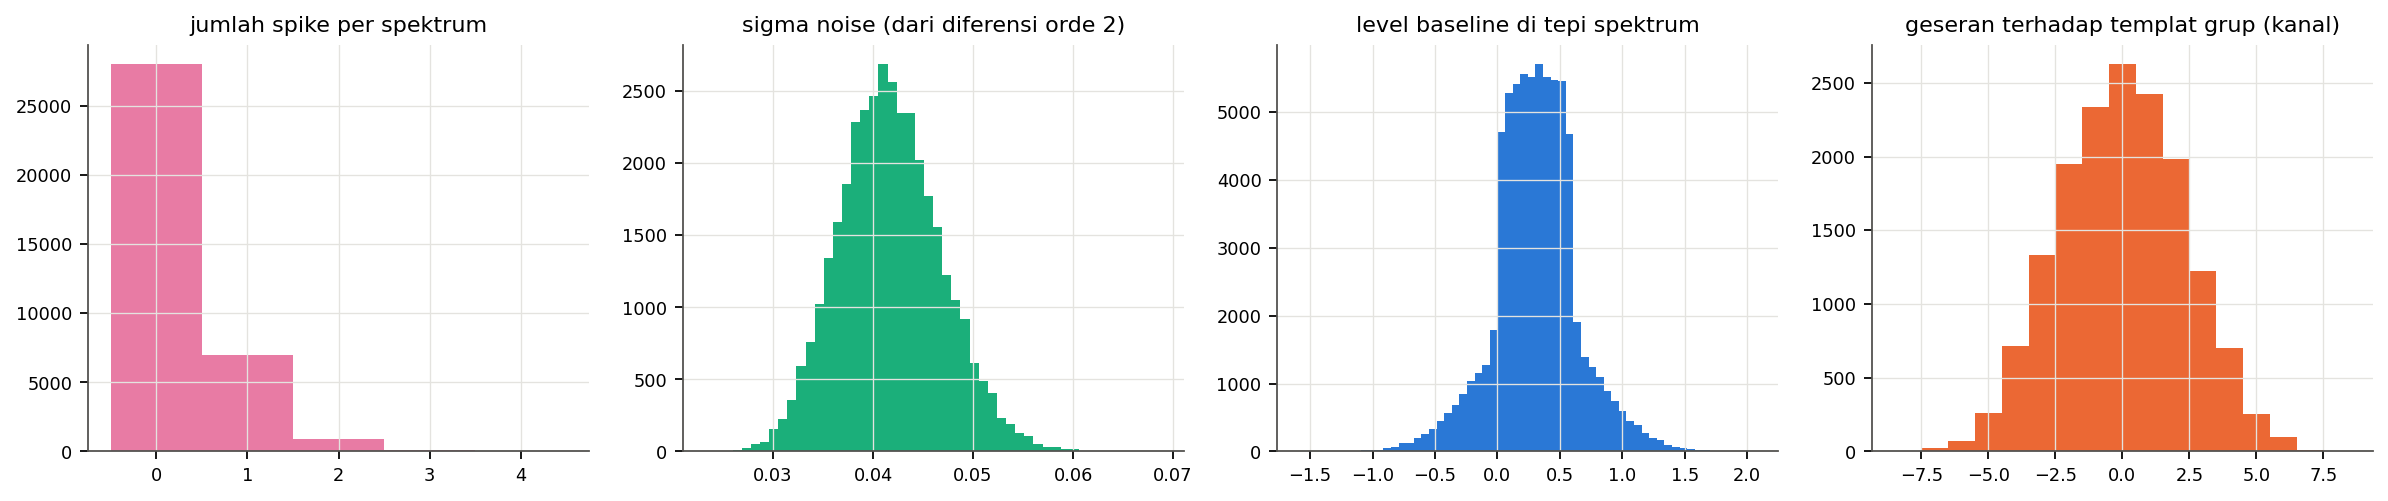
\includegraphics[width=\linewidth]{t3_eda_spectrum_distortions}
  \caption{Spectrum distortions: spikes (22.2\% of samples), baseline offset/tilt, and wavelength shift.}
  \label{fig:t3-eda-spec}
\end{figure}

\begin{figure}[!htbp]
  \centering
  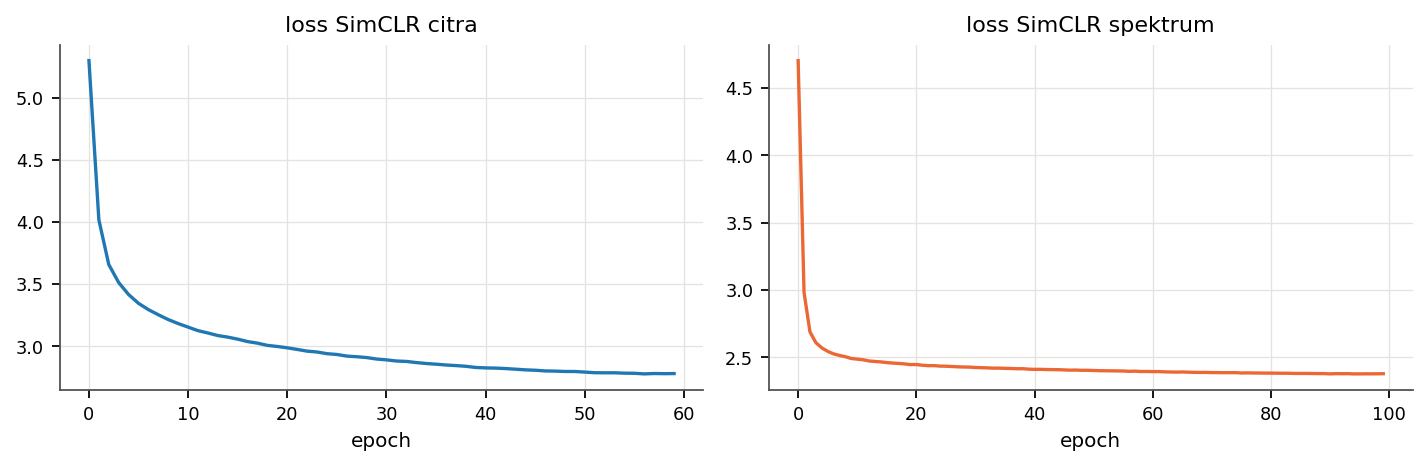
\includegraphics[width=\linewidth]{t3_simclr_loss}
  \caption{SimCLR NT-Xent training loss curves for the image (60 epochs) and spectrum (100 epochs) encoders.}
  \label{fig:t3-loss}
\end{figure}

\begin{figure}[!htbp]
  \centering
  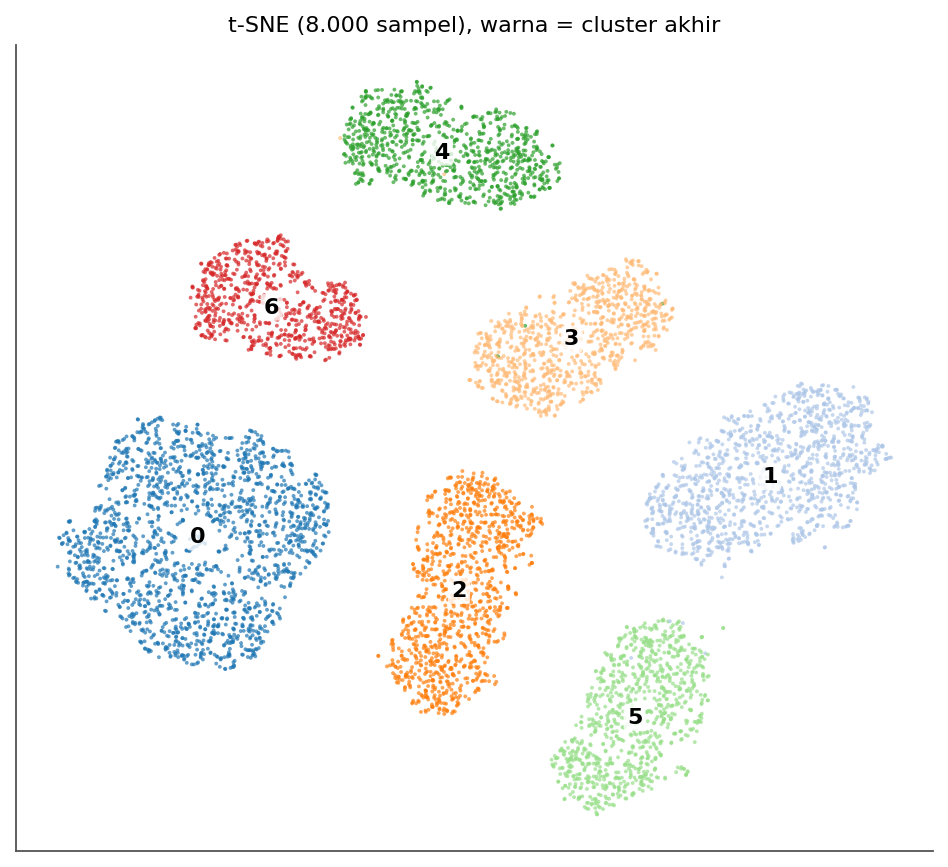
\includegraphics[width=\linewidth]{t3_tsne_clusters}
  \caption{t-SNE~\cite{vandermaaten2008tsne} projection of the fused \texttt{concat} embedding coloured by final cluster ID (0--6).}
  \label{fig:t3-tsne}
\end{figure}

\begin{figure}[!htbp]
  \centering
  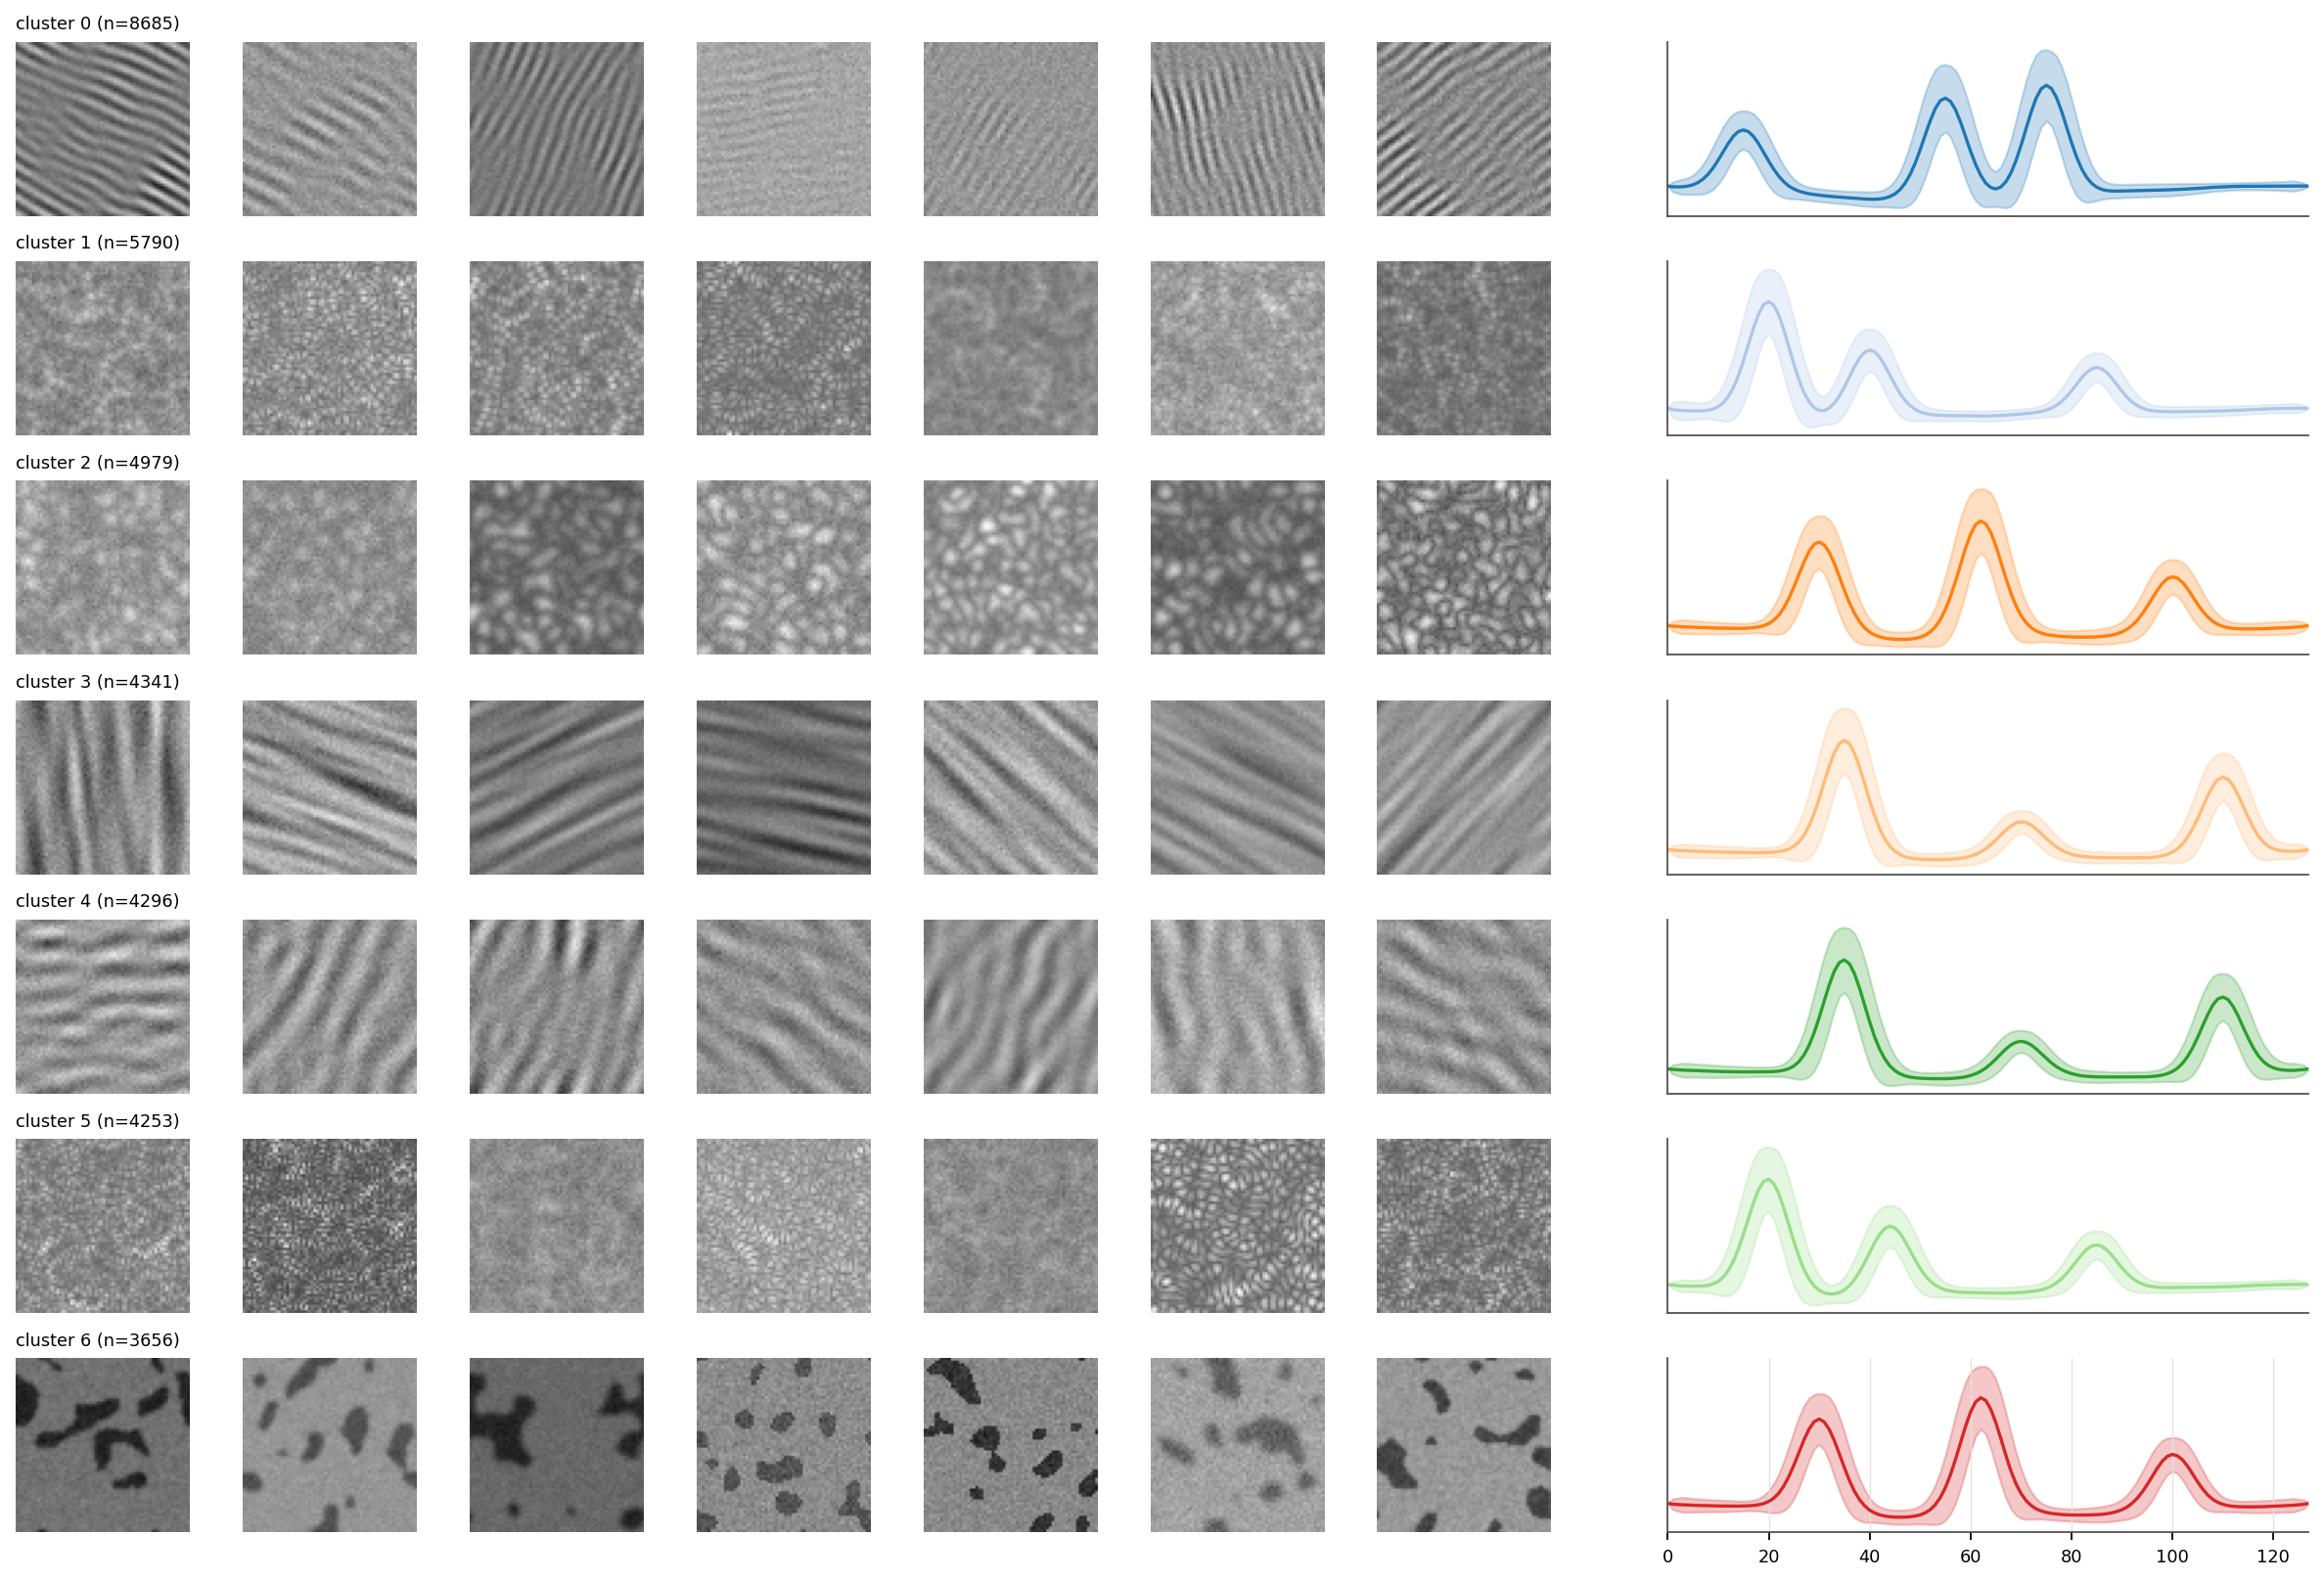
\includegraphics[width=\linewidth]{t3_cluster_profiles}
  \caption{Representative microstructure images and mean preprocessed spectra for each of the 7 clusters.}
  \label{fig:t3-profiles}
\end{figure}



\end{document}
